

In this chapter a short overview on the basic concepts of Convolutional Neural Networks (CNNs) will be given. 
The scope is to give the necessary background for the understanding of the structure and the motivations behind the 
Deep Learning (DL) models employed for the analysis of BCDI data, presented in the next chapters.  

For more comprehensive and exhaustive dissertations about Machine Learning (ML) and Artificial Neural Networks (ANNs)
the book of Goodfellow \cite{Goodfellow_2016} and the more recent from Prince \cite{prince2023understanding} are 
suggested to the reader. 

ANNs is a type of machine learning algorithm inspired by the biological neuron structure. ANNs are generally composed of interconnected 
nodes where the signal is processed through operations with tunable parameters named weights 
and biases for multiplications and addition respectively. Important feature of each node is the \textit{activation function}, 
that introduces a non-linear operation and returns the node's output \cite{jagtap2022}. Several kinds of these 
activation functions exist and their use depends on the properties of each (bounds, derivatives, positivity, etc.) 
\cite{kunc2024}. In the following chapters the modified rectifying linear unit, known as LeakyReLU \cite{Maas2013RectifierNI}, 
and the sigmoid, also known as logistic, function will be used. Neurons are generally organized into \textit{layers} and 
are connected between neurons of other layers. In \textit{feed-forward} neural networks the information flows from the 
input layer to the output layer with forward connections only.
In other neural networks, like \textit{recurrent} ones, the connections are also designed backwards. 

\begin{figure}[H]
    \centering
    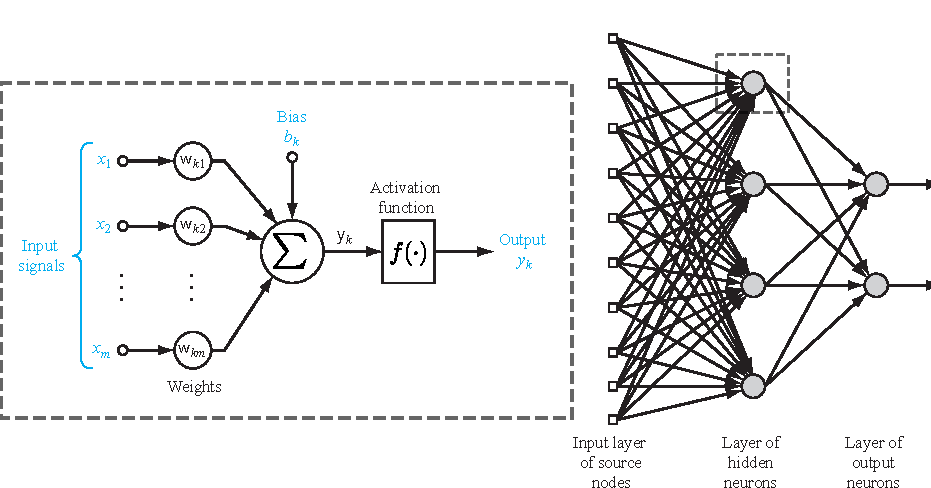
\includegraphics[width=\textwidth]{figures/Intro/neuron2.pdf}
    \caption{\textbf{Schematic of an artificial neuron and a neural network.} On the left, a series of input signals 
    $x_i$ are multiplied by the tunable weight $w_{k}$ and summed together with the tunable bias $b_k$ relative to 
    the $k$-th neuron. The output is then passed through the activation function $f$ which produce an output $y_k$ 
    which is a non-linear combination of the inputs. On the right, the feed-forward network composed of two \textit{hidden}
    layers of artificial neurons processing the ten units long vector $x$ and returning a binary output.
    Adapted from \cite{haykin2009neural}}
    \label{fig:neuron}
\end{figure}

The use of non-linear functions is found to be fundamental for the powerful analytical and statistical properties of ANNs, 
which have been progressively 
established over the years. It was shown \cite{Cybenko1989, Hornik_1989, Leshno_1993} that ANNs with appropriate 
activation functions and sufficient parameters can approximate any continuous function on a compact domain to arbitrary 
accuracy (\textit{universal approximation theorems}). 

Typically, one seeks the combination of parameters $\theta_k = (w_k, b_k)$ of the neural network $\mathcal{N}_{\theta}$ 
such that $\mathcal{N}_{\theta}$ well approximates the unknown mapping $\mathcal{M}$ between an input $x$ and the output 
$y = \mathcal{M}(x)$.  

At this point one can ask: How is this mapping found? The core idea is known as Empirical Risk Minimization and states that 
when the $\theta_k$ are adjusted to fit a sufficiently large dataset consisting of samples drawn from an underlying distribution, 
the function being approximated reflects the statistical relationships encoded in that distribution \cite{Hornik_1990}.
By the Law of Large Numbers, the empirical distribution observed in the \textit{training set} converges to the true 
distribution as the sample size grows, and thus the empirical risk minimized during training approaches the true 
risk. This statistical foundation explains why ANNs are able to generalize to new, unseen data drawn from the 
same population. 

Formally, we can consider $X$ as the set of all events belonging to the same statistical distribution and 
$Y$ similarly. The mapping $\mathcal{M}$ is known for a limited set of examples $(x_1,y_1 = \mathcal{M}(x_1)), ..., 
(x_n, y_n = \mathcal{M}(x_n))$. This set is known as training set where each $x_i$ is an input instance and $y_i$ the 
corresponding ground truth transformation operated by $\mathcal{M}$. We can now introduce a non-negative scalar 
real-valued \textit{loss function} $L(\hat{y},y )$ which measures the difference between the ground truth $y$ and the 
output of the neural network $\hat{y} = \mathcal{N}_\theta (x)$ for each element of the training set. 
It follows that having the best approximation of the mapping $ \mathcal{N}_\theta \approx \mathcal{M}$ is obtained when 
the score of the loss function averaged across the number of training samples is lowest. 
The problem of approximating the mapping between the input and ground truth in the training set is then formulated as 
minimization problem of the type: 
\begin{equation}
    \mathcal{N}_\theta = \argmin{\theta} L
\end{equation}
 

% 

\section{Motivation: CNN for Inverse Problems}
A CNN is a type of \textit{deep} ANN in which the convolution operation is repeatedly applied to the signal. 




\section{Principles and building blocks}\label{chp:cnn}
\subsection{Convolutional Layer}
\subsection{Pooling Layer}
\subsection{Activation Layer}

\section{U-Net and MSD-Net}
% use skip connections

\section{Training}
\subsection{Automatic differentiation and Backpropagation}
\subsection{Stochastic Gradient Descent}
